%\documentclass[10pt,handout]{beamer}
\documentclass[10pt]{beamer}
\usetheme[white]{Wisconsin}
%\title[short title]{long title}
\title{\large Spent Nuclear Fuel Attribution using Statistical Methods}
%\subtitle[short subtitle]{long subtitle}
\subtitle{Impacts of Information Reduction on Prediction Performance}
%\author[short name]{long name}
\author{Arrielle Opotowsky \\ \vspace{4mm} PhD Defense, Advised by Paul P.H. Wilson}
%\date[short date]{long date}
\date{16 August 2021}
%\institution[short name]{long name}
\institute{University of Wisconsin-Madison}

\usepackage{hyperref}
\usepackage{enumerate}
\usepackage{amsmath}
\usepackage{amssymb}
\usepackage{multicol}
\usepackage{lmodern}
\usepackage[LY1]{fontenc}
\usepackage{mathtools}
\usepackage{changepage}
\usepackage{tabularx}
\usepackage{booktabs}
\usepackage{multirow}
\usepackage{colortbl}
\setbeamertemplate{footline}[frame number]
\setbeamertemplate{bibliography item}[text]
\setbeamercolor{page number in head/foot}{fg=gray}
\setbeamercovered{transparent}

% thanks to katy huff: get rid of header on title page\dots
\makeatletter
    \newenvironment{withoutheadline}{
       \setbeamertemplate{headline}[default]
       \def\beamer@entrycode{\vspace*{-\headheight}}
    }{}
\makeatother

% highlight words
\setbeamercolor{alerted text}{fg=black,bg=lightgray}
\newcommand{\boxalert}[1]{{%
  \usebeamercolor{alerted text}\colorbox{bg}{\alert{#1}}%
}}

% bold text in math environment
\newcommand\allbold[1]{{\boldmath\textbf{#1}}}

\begin{document}
%%%%%%%%%%%%%%%%%%%%%%%%%%%%%%%%%%%%%%%%%%%%%%%%%%%%%%%%%%%%%
%% From uw-beamer Here's a handy bit of code to place at 
%% the beginning of your presentation (after \begin{document}):
\newcommand*{\alphabet}{ABCDEFGHIJKLMNOPQRSTUVWXYZabcdefghijklmnopqrstuvwxyz}
\newlength{\highlightheight}
\newlength{\highlightdepth}
\newlength{\highlightmargin}
\setlength{\highlightmargin}{2pt}
\settoheight{\highlightheight}{\alphabet}
\settodepth{\highlightdepth}{\alphabet}
\addtolength{\highlightheight}{\highlightmargin}
\addtolength{\highlightdepth}{\highlightmargin}
\addtolength{\highlightheight}{\highlightdepth}
\newcommand*{\Highlight}{\rlap{\textcolor{HighlightBackground}{\rule[-\highlightdepth]{\linewidth}{\highlightheight}}}}
%%%%%%%%%%%%%%%%%%%%%%%%%%%%%%%%%%%%%%%%%%%%%%%%%%%%%%%%%%%%%
%%--------------------------------%%
\begin{withoutheadline}
\frame{\titlepage}
\end{withoutheadline}

%%--------------------------------%%
%\AtBeginSection[]{
%\begin{frame}
%  \frametitle{Outline}
%  %\begin{multicols}{2}
%    \centering
%    \tableofcontents[currentsection,currentsubsection]
%  %\end{multicols}
%\end{frame}
%}

\AtBeginSubsection[]{
\begin{frame}
  \frametitle{Outline Progress}
  \begin{center}
    \begin{minipage}{0.85\textwidth}
      \tableofcontents[currentsection,currentsubsection]
    \end{minipage}
  \end{center}
\end{frame}
}

\section{Introducing Nuclear Forensics and Statistical Methods}
\subsection{Motivation}
\begin{frame}
  \frametitle{Needs in Nuclear Forensics}
  Should find or make a figure representing a general explanation of this field
\end{frame}

\begin{frame}
  \frametitle{Contribution of Statistical Methods}
  \begin{figure}[h!]
    \centering
    \includegraphics[width=0.9\textwidth]{CompStatForensicsWorkflow.png}
    \caption{Nuclear forensics research via computational workflows}
  \end{figure}
\end{frame}

\subsection{Background}

\begin{frame}
  \frametitle{Pre-detonation Nuclear Forensics Investigations}
  \begin{adjustwidth}{-15pt}{-15pt}
  \begin{figure}
    \centering
    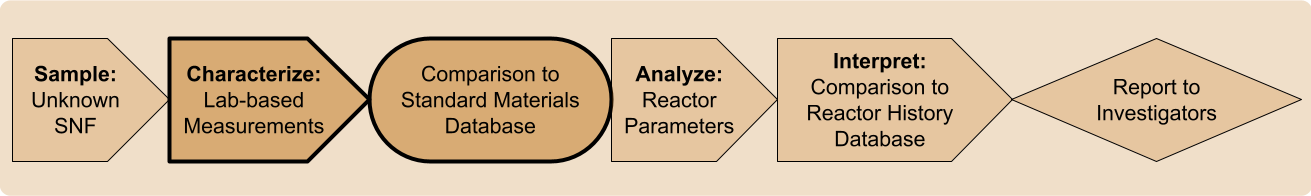
\includegraphics[width=1.1\textwidth]{./figures/forensicsrealworld.png}
  \end{figure}
  \vspace{6mm}
  \hspace{10mm}
  \begin{minipage}{0.85\linewidth}
    \begin{itemize}
      \item<1-> Collection: depends on intercepted material
      \item<2-> Characterization: non-destructive and destructive
      \item<3-> Goals:
      \begin{itemize}
        \item Inverse problem: reactor of origin, material chain of custody
        \item Safety: material handling and security
      \end{itemize}
      \item<4-> Data evaluation
    \end{itemize}
  \end{minipage}
  \end{adjustwidth}
\end{frame}

\begin{frame}
  \frametitle{Attributing Spent Nuclear Fuel}
  \setbeamercovered{}
  \begin{enumerate}
    \onslide<1->{
    \item \textbf{Reactor Type} \\
          Classified as one of three common types of commercial power reactors:
          \begin{itemize}
            \item Pressurized water reactor (PWR)
            \item Boiling water reactor (BWR)
            \item Pressurized heavy water reactor (PHWR)
          \end{itemize}
    }
    \onslide<2->{
    \item \textbf{Burnup} \\
          How much energy was produced by the fuel: megawatt-days (or 
          gigawatt-days) per metric ton of initial uranium: $\mathbf{MWd/MTU}$ 
          ($GWd/MTU$)
    }
    \onslide<3->{
    \item \allbold{${}^{235}\text{U}$} \textbf{Enrichment} \\
          Percentage of ${}^{235}\text{U}$ with respect to total uranium in 
          fuel: \allbold{$\%\:{}^{235}\text{U}$}
    }
    \onslide<4->{
    \item \textbf{Time Since Irradiation} \\
          How long fuel has been out of reactor core (aka cooling time): 
          $\mathbf{days}$ or $years$
    }
  \end{enumerate}
\end{frame}


\begin{frame}
  \frametitle{Machine Learning Approach}
  \begin{adjustwidth}{-10pt}{-10pt}
  \begin{figure}
    \centering
    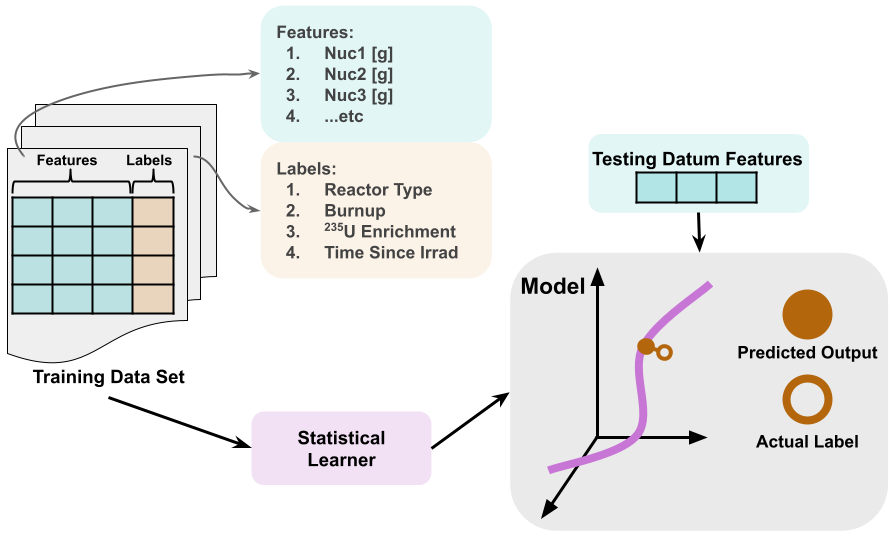
\includegraphics[width=1.05\textwidth]{./figures/pres_version_SupervisedRegression.png}
  \end{figure}
  Training and predicting using supervised regression (classification not shown)
  \end{adjustwidth}
\end{frame}



\section{Experimental Methodology}
\subsection{Overview \& Methodology Development}

\begin{frame}
  \frametitle{Computational Methods}
  \begin{figure}[h!]
    \centering
    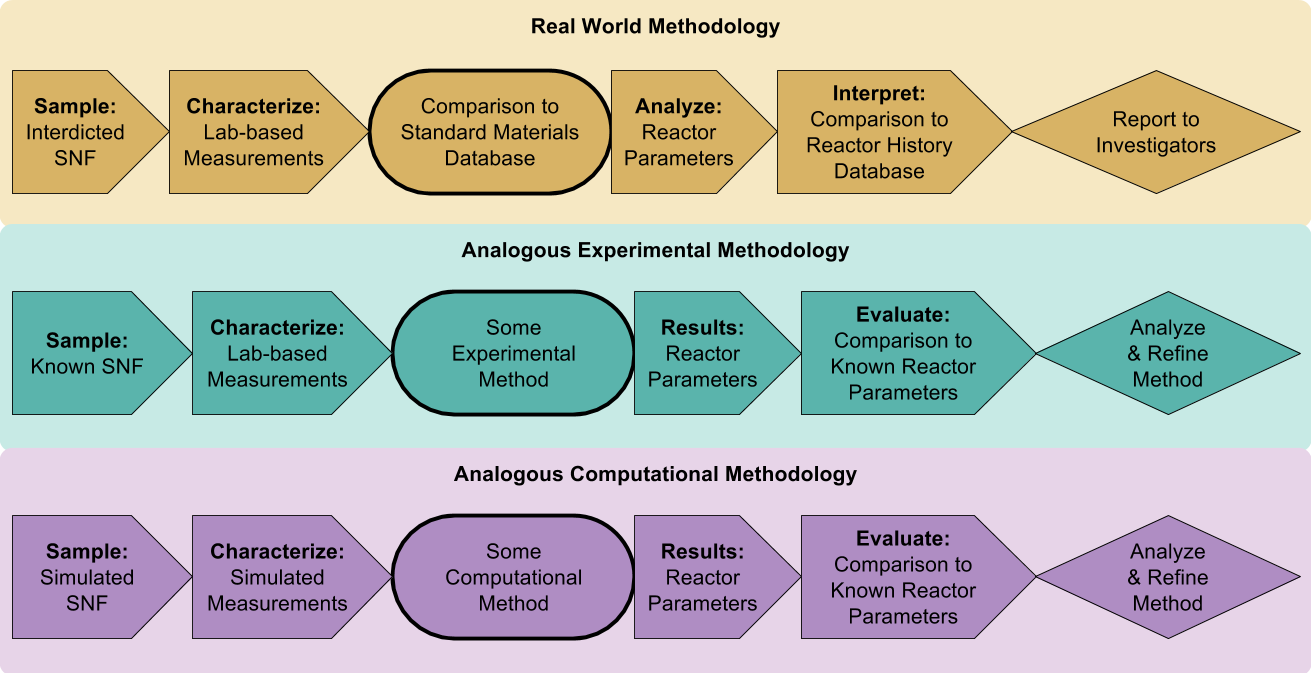
\includegraphics[width=0.9\textwidth]{./figures/ForensicsWorkflows.png}
    \caption{Nuclear forensics research: physical, experimental, and computational}
  \end{figure}
\end{frame}

\begin{frame}
  \frametitle{Computational Methods}
  \begin{figure}[h!]
    \centering
    \includegraphics[width=0.9\textwidth]{./figures/CompStatForensicsWorkflow.png}
    \caption{Comparison of two different computational approaches}
  \end{figure}
\end{frame}

\begin{frame}
  \frametitle{Statistical Methods}
  \begin{minipage}{0.5\textwidth}
    \begin{figure}
      \centering
      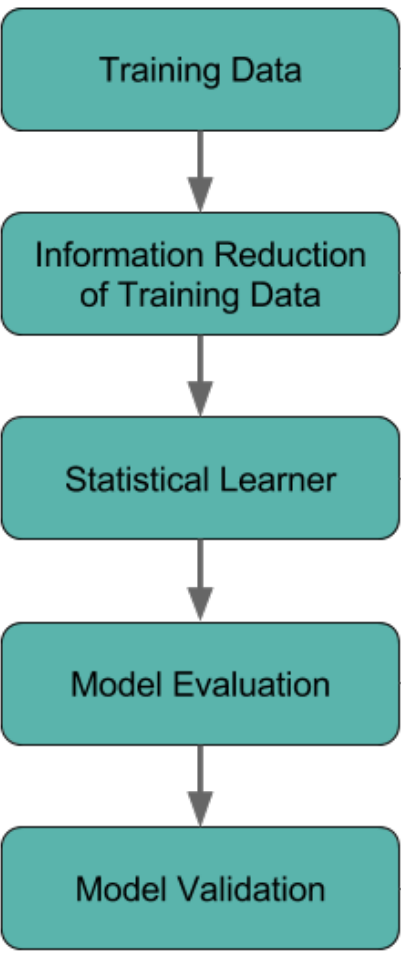
\includegraphics[height=0.6\textheight]{./figures/statmethodology.png}
      \caption{Workflow of a  methodology using statistical models}
    \end{figure}
  \end{minipage}%
  \begin{minipage}{0.5\textwidth}
    \begin{itemize}
      \item Training data: large set of SNF measurements
      \begin{itemize}
        \item Labels (e.g., burnup)
        \item Features (e.g., nuclide concs)
        \item Instances (individual SNF recipe)
      \end{itemize}
      \item Statistical learner
      \begin{itemize}
        \item Machine learning algorithms
        \item Algorithm parameters
        \item Predict label of new instance
      \end{itemize}
      \item Model evaluation
      \begin{itemize}
        \item Diagnostic curves
        \begin{itemize}
          \item Learning curves
          \item Validation curves
        \end{itemize}
        \item Prediction error
        \begin{itemize}
          \item Bias versus variance
          \item Generalizability
        \end{itemize}
      \end{itemize}
    \end{itemize}
  \end{minipage}
\end{frame}

\begin{frame}
  \frametitle{Statistical Methods}
  \begin{figure}[h!]
    \centering
    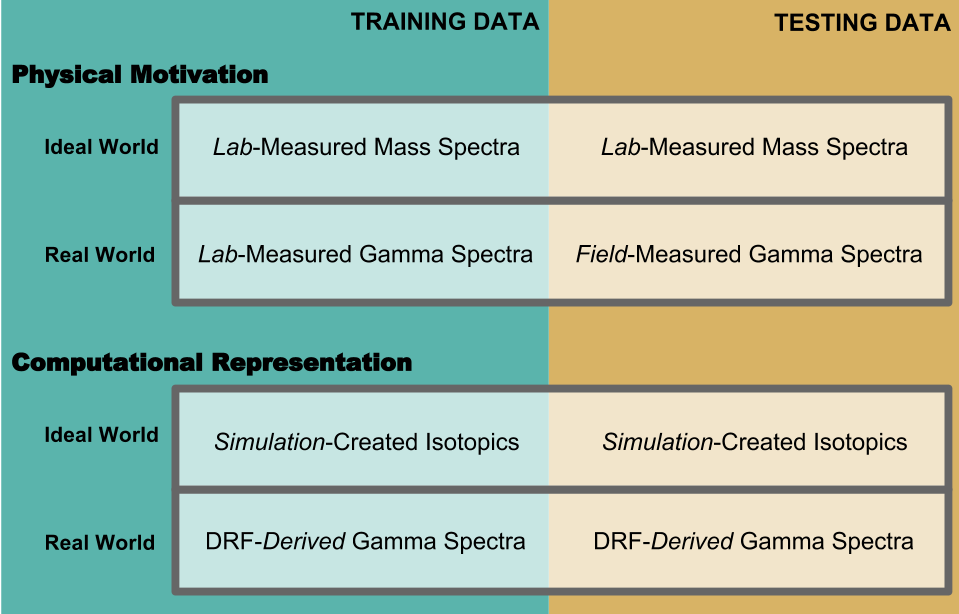
\includegraphics[width=0.75\textwidth]{./figures/proposal.png}
    \caption{Illustration of data set modularity}
  \end{figure}
\end{frame}


\subsection{Training Database Simulation}
\begin{figure}[H]
  \centering
  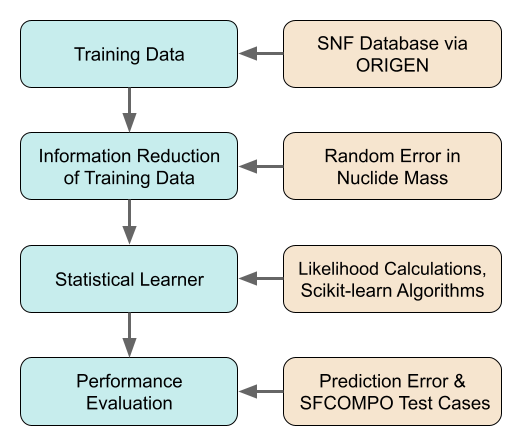
\includegraphics[width=0.7\linewidth]{./chapters/exp1/methodology1.png}
  \caption{First portion of the flowchart from Figure \ref{fig:method} being 
           described in this section.}
\end{figure}

Of interest to an entity trying to create a weapon is partially irradiated fuel
if they have plutonium separations capabilities or any radioactive substance in
the case of a dirty bomb. Thus, this work focuses on \gls{SNF} from commercial
power reactors. Ideally, a large enough database of \gls{SNF} nuclide assays
would be able to be used for this work. Since that does not exist, the 
database will be simulated via \gls{ORIGEN-ARP} \cite{origen, origenarp}.  

\subsection{Simulation Fidelity}
\label{sec:fidelity}

Nuclear fuel cycle studies involve tracking the material flow of nuclear fuel.
This can be anywhere from mining to waste management, or focus on a process
step in between. Fuel cycle studies are not necessarily nuclear-specific. For
example, they can be used to evaluate economic predictions, environmental
impact, transportation planning, etc.  In order to draw conclusions from these
studies, it is common to use a nuclear fuel cycle simulator that tracks the
quantities of interest. These allow the comparison of different fuel types,
reactor technologies, material processing steps, etc. 

There are simplifications researchers need to make in order to experiment in a
controlled way. Fuel cycle simulators, built for a specific needs, must remove
complicating factors that are less relevant to the study.  For example, one
tool might be suited well to large-scale systems analysis with little nuclear
physics included in the models, and another might focus on detailed isotopics
within a system to track plutonium.

Because a large portion of a nuclear forensics investigation relies on
measuring isotopics, this work used \gls{ORIGEN} \cite{origen}, which is a part
of the \gls{SCALE} 6.2 modeling and simulation suite of computational tools
developed for nuclear design and safety \cite{scale}. \gls{ORIGEN} was chosen
for its physically detailed models of activation, depletion, and decay.
Specifically, the ARP module of the code was used: \gls{ORIGEN-ARP}
\cite{origenarp}.

\gls{ORIGEN} calculates time-dependent nuclide concentrations (or quantities
derived from these) that result from activation and depletion calculations. The
physics (i.e., neutron transport and decay) calculations are carried out in
other \gls{SCALE} modules that solve the depletion equations.  This generates
libraries for \gls{ORIGEN} that include the probabilities of reaction (i.e.,
cross sections) for the system.

To obtain an \gls{SNF} recipe from a reactor simulation, \gls{ORIGEN} uses the
desired input power generation with the cross section library to calculate a
flux, the resulting depletion, and the end composition (i.e., isotopic recipes
or nuclide vectors).  Another output is decay; the composition is computed
using decay equations with nuclear data \cite{endf}. These compositions provide
source terms for other calculations, such as decay emission spectra from
neutrons, alpha particles, beta particles, and gamma rays. Other derived
quantities like activity, decay heat, or radiological hazard factors are also
an option.

\gls{ORIGEN-ARP} allows users to access a wider range of simulations by
interpolating between the pre-calculated libraries instead of creating new
libraries.  It is known to be validated for \gls{LWR} \gls{SNF}
\cite{lwr_valid}. Additionally, recycled \gls{SNF} in the form of mixed oxide
fuel has been benchmarked for the relevant reactors \cite{mox_valid}.  Through
\gls{ORIGEN}, given an initial material composition, some reactor operation
parameters, and a reactor type, one can quickly perform many different nuclear
reactor simulations and obtain \gls{SNF} recipes.

\todo[inline]{This section needs more information about ORIGEN-ARP validation
and maybe some nuclides that are known to perform poorly from ARP sims. Can
show a generic example from one of my sources, and or an example of trying to
match an ORIGEN-ARP simulation to an SFCOMPO entry. It is important to inform
that this training set as ground truth is not perfect truth, for some nuclides
more than others. The goal is to explain the ARP validation without getting
too deep.  This tool was necessary for the 500k training set. The prediction
performance will be impacted by the poorly simulated nucs, so it may be
worthwhile to note which ones have consistently large sim errors (unless this
involves getting too deep). P.S. did you mention homogenized core above?}

\subsection{Training Set Labels}
\label{sec:snflbls}

\begin{table}[!htb]
  \centering
  \begin{subtable}{\linewidth}
    \centering
    
\includegraphics[width=0.5\linewidth]{./chapters/exp1/trainset4_Orxtrs.png}
    \caption{\gls{ORIGEN} designations for reactor technologies and fuel assembly design.}
    \label{tbl:rxtrtype}
    \vspace*{5mm}
  \end{subtable}
  \begin{subtable}{\linewidth}
    \centering
    
\includegraphics[width=0.75\linewidth]{./chapters/exp1/trainset4_inputs.png}
    \caption{Simulation parameters for \gls{ORIGEN} input files.}
    \label{tbl:rxtrparam}
  \end{subtable}%
  \caption{Training set database design using the \gls{SFCOMPO} database as guidance. \cite{sfcompo}}
  \label{tbl:train}
\end{table}

The design of the training set is dependent on a number of factors.  First, it
must have a sufficient number of burnup sets and time since irradiation steps
to provide robust prediction. This is decided upon by maximizing the steps for
both parameters, while balancing the computational limitations of a large
training set. Through previous experience, an approximate limit would be around
$1e6$ database entries for the specific calculations in this work and employing
reasonable computational limitations.

Secondly, the training set must represent what exists in the real world. This
was accomplished by studying the spread of parameters in the \gls{SFCOMPO}
database \cite{sfcompo}.  To ensure this, a variety of reactor types and
assembly designs were included, listed in Table \ref{tbl:rxtrtype}. Table
\ref{tbl:rxtrparam} lists the rest of the simulation inputs. These include not
only the labels of prediction interest, \gls{U235} enrichment, burnup, and time
since irradiation, but also other important simulation input parameters such as
the reactor power density and the moderator density.  (Water is both the
moderator and coolant in all simulated reactor types.)

\begin{figure}[!hbt]
  \makebox[\textwidth][c]{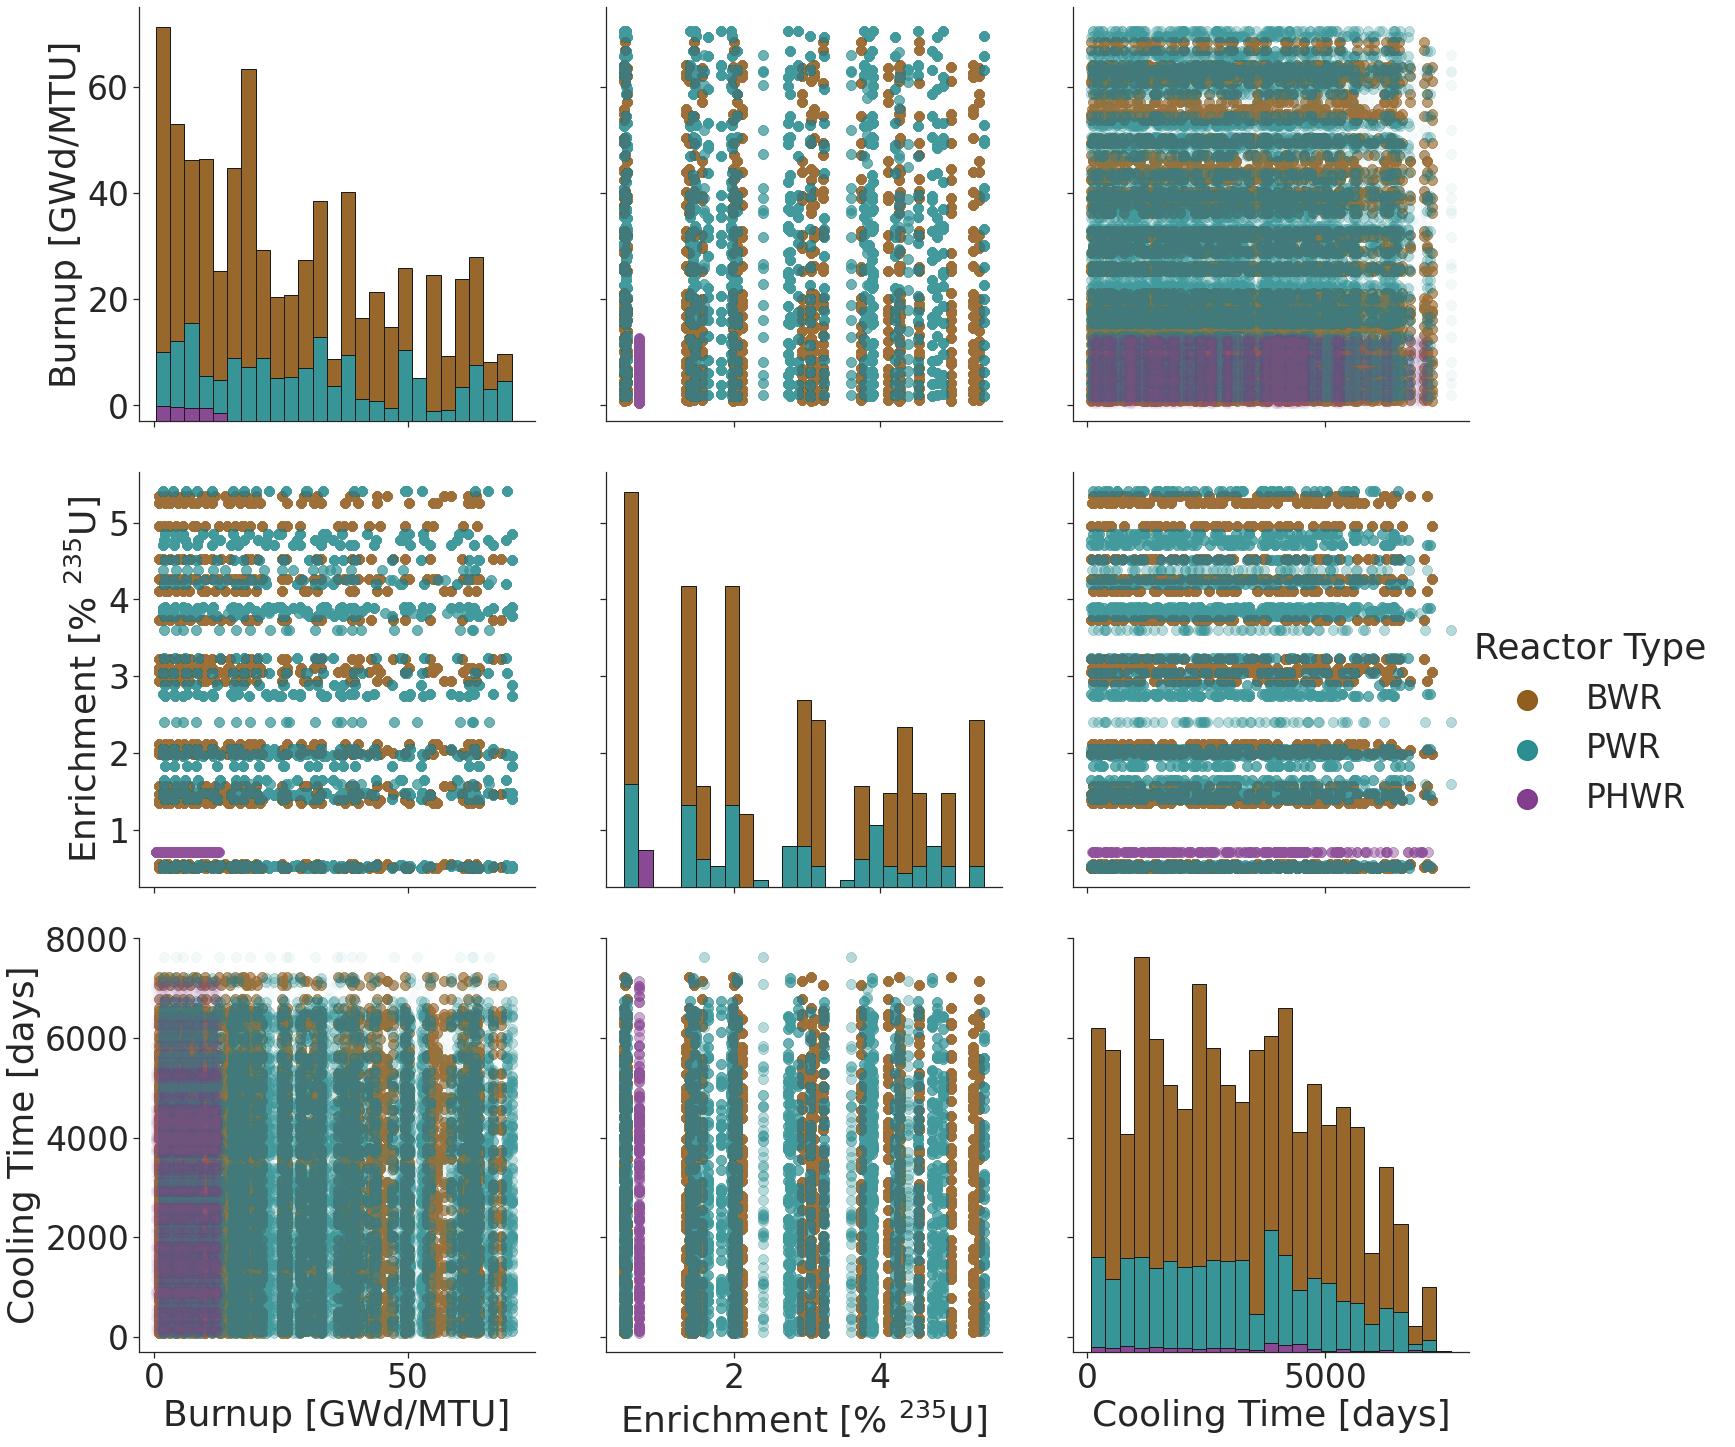
\includegraphics[width=\linewidth]{./chapters/exp1/histogram_scatter_trainset_viz.png}}
  \caption{A combination of histograms and scatter plots to visualize the 
           distribution of prediction labels in the training set.}
  \label{fig:trainhist}
  \todo[inline]{fix the histogram figure, this is a placeholder}
\end{figure}

The third factor influencing database design is ensuring ideal \gls{ML}
algorithm performance.  As mentioned in Section \ref{sec:errs}, many algorithms
are developed with the assumption that the training set will be
\acrfull{i.i.d.}.  This is important so that the model does not overvalue or
overfit a certain area in the training space. With the training set design,
there are predetermined values for enrichment, burnup, and time since
irradiation.  While there are $21-28$ burnup steps (depending on the reactor
type) and 61 cooling time steps, there are only 6 values for enrichment. This
creates the risk that the algorithm will end up being unable to generalize
outside of those discrete values. Therefore, the burnup steps and time steps
are perturbed randomly in a range that is $\pm10\%$ and $\pm30\%$ from the
originally defined values, respectively.  The enrichment also gets perturbed by
$\pm10\%$, and not more because the cross-section libraries in \gls{ORIGEN-ARP}
are pre-calculated for those enrichment values, so deviating too far from them
would result in inaccurate \gls{SNF} simulations. The power densities and
moderator densities were kept at the values defined in Table
\ref{tbl:rxtrparam}.  The resulting training set is $450240$ (or $4.5e5$)
entries.  Figure \ref{fig:trainhist} visualizes the somewhat even distribution
of the burnup and cooling time parameters, and shows the lack of even
distribution of the enrichment parameter through a combination of scatter plots
and histograms.  Note that there are many more \gls{BWR}s present in the
histograms because of the multiple moderator densities simulated (see Table
\ref{tbl:rxtrparam})

\subsection{Training Set Features}
\label{sec:snffeats}

The other design decision regarding the training set is related to
which nuclides to track, i.e., the features.  For this experiment, nuclide
masses are necessary, and the most common measurements in \gls{SFCOMPO} guide
the list of nuclides tracked.  

The set of training features of 29 nuclide masses listed in Table
\ref{tbl:nucmass} was designed with the following reasons in mind.  First, the
units in mass is to represent the scenario of "perfect knowledge", where a full
assay is done via mass spectrometry techniques.  Second, this is to have the
training set units convertable to those present in the external, real-world
test set: the \gls{SFCOMPO} database.  The \gls{ORIGEN} simulations output the
nuclide masses in $grams$, and they are converted to the units of
\textit{milligrams per gram of initial uranium}, $mg/gU_i$, when the models are
externally tested against \gls{SFCOMPO}. Lastly, the 29 nuclides chosen were
based on the presence of measurements in \gls{SFCOMPO}, where these were
present in at least 100 of the samples in the database.  The external test set
is described in more detail in Section \ref{sec:sfcompo}.

\begin{table}[!htb]
  \centering
  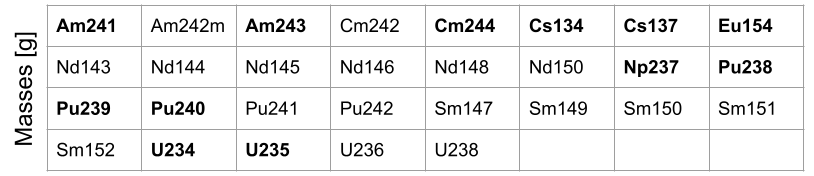
\includegraphics[width=\linewidth]{./chapters/exp1/nucmass_feats.png}
  \caption{Set of features saved for the first experiment, nuclide masses 
           measured in $grams$. The bold nuclide masses overlap with the 
           nuclides in \ref{tbl:nucacts}.}
  \label{tbl:nucmass}
\end{table}


\subsection{Statistical Methods Overview}
%\setlength\abovedisplayskip{2.5pt}

For relevant nuclear forensics predictions, both classification and regression
algorithms must be used.  For example, one may want to predict the reactor type
label given some measurement-based features of \gls{SNF} of an unknown source.
This would require a classification algorithm. Or perhaps the input fuel
composition is relevant to an investigation on weapons intent, so a regression
algorithm would be used. 

There are three algorithms presented in this section: \textit{k}-nearest
neighbors, decision trees, and \gls{MLL} calculations. They were chosen based
on their simplicity; this work has yet to be benchmarked using simple
algorithms so a more complex treatment of the training sets in this work would
be premature. Additionally, in part because of their simplicity, they are all
"white box" methods.  This is unique in the \gls{ML} universe, since most
algorithms create a black box model that is unable to be analyzed by a human.
The  decision trees method provides an output model that can be used to discern
behavior and understand predictions, and \textit{k}-nearest neighbors and
\gls{MLL} calculations do not create a model at all. Individual predictions can
still be analyzed, however, since the procedures are so simple. 

\subsubsection{Nearest Neighbor Methods}

Nearest neighbors classification and regression are unique algorithms in
that thay are instance-based; they do not actually generalize, but instead
track the observations in the training set.  The main metric for this algorithm
is distance (or dissimilarity) between the test sample and the closest training
sample(s) in the vicinity.  During prediction, the algorithm will calculate a
value based on the instance that is closest to the current test sample. Thus,
there is not any learning, but instead a direct comparison between an unknown
sample and the space that the training set populates. The predictions from
nearest neighbors can be quite accurate, but are highly unstable to
peturbations \cite{elements_stats}.

The process of prediction with \textit{k}-nearest neighbors is as follows.
First, the distances between the test sample and each of the training set
instances are calculated.  Most commonly the Euclidian distance is used, but
this walkthrough uses the Manhattan distance:
\begin{equation}
  d_{i} = \sum_{j=1}^{N_{feats}} |x_{j,train} - x_{j,test}|
  \label{eq:l1}
\end{equation}
where $i$ is each training set instance, and $j$ refers to each feature in the
training set.  The lowest \textit{k} $d_{i}$ are chosen. For \textit{k}-nearest
neighbors regression, the value, $y$ is predicted using the following equation.
\begin{equation}
  y(\boldsymbol{x}) = \frac{1}{k} \sum_{i=1}^{k} w_i \cdot y_i
  \label{eq:knn}
\end{equation}
where $w_{i}$ is either uniform and takes on a value of $1$ or is
distance-based and takes on a value of $1/d_{i}$ and $\boldsymbol{x}$ is the
full set of features. The regression equation averages the closest \textit{k}
neighbors for an estimate of the unknown sample.  In \textit{k}-nearest
neighbors classification, the class label $y$ is predicted using the mode of
the nearest neighbors selected using the \textit{k} smallest $d_i$, or when
$w_i$ is $1/d{i}$ the weighted mode is used to choose the predicted label.

\begin{figure}[!htb]
  \centering
  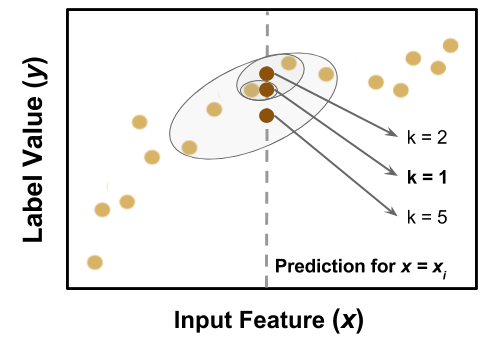
\includegraphics[width=0.8\linewidth]{./chapters/litrev/nn-fig.png}
  \caption{Schematic of \textit{k}-nearest neighbors regression, showing how 
           changing \textit{k} alters the predicted label value $y$.}
  \label{fig:nn}
\end{figure}

Figure \ref{fig:nn} provides a pictoral explanation of Equation \ref{eq:knn}
for a prediction where there is one feature. In this figure, there is a test
sample with a feature, valued at $x_i$, indicated with the grey dotted line.
The three circles represent the neighborhood given by the value of \textit{k},
and the darker dots on the line represent the reported prediction $y$ for each
choice of \textit{k}.  In this illustration, $k=1$ or $k=2$ provide a more
accurate prediction according to a visual inspection of the trend, but higher
values of $k$ can be useful, and will be discussed in Section
\ref{sec:complexity}.

\subsubsection{Decision Trees}

Decision trees are a common choice because they are simple to implement and
provide an interpretable model. However, the predictions from decision trees,
similar to \textit{k}-nearest neighbors, are unstable to peturbations.  What
follows is a highly simplified explanation of the Classification and Regression
Trees algorithm for growing decision trees, showing only the equations for
splitting criteria.  A more complete treatment can be found in Reference
\cite{elements_stats} or in the User Guide in Reference \cite{scikit}.

At their core, decision trees algorithms split the feature space into different
regions.  Decision trees are constructed by iteratively finding places in the
feature space at which to split the data to best predict a label. Some measure
of information gain (more accurately the opposite, impurity, denoted here as
$H$) is used to select a splitting criterion at each split, which maximizes
differentiation between average label values in regression or groups similar
labels together in classification.  This process continues until some
externally set stopping requirement is met, or no information gain can be made
by continuing to create splits. 

Each split creates two new nodes on the tree, where the node has to find a new
splitting criterion. In the math that follows, there are nodes given by $m$,
and a number of samples in each node given by $N_{\text{samples}, m}$. The
individual node samples are given by $i$. The impurity at the node is denoted
as $H(m)$. In classification, the node impurity can be measured by the Gini
index, where $p_{m, k}$ is the proportion of class $k$ observations at the
node:
\begin{equation}
  \begin{aligned}
    p_{m, k} &= \frac{1}{N_{\text{samples}, m}} \sum_{i=1}^{N_{\text{samples}, m}}
              I(y = k)
    \\
    H(m) &= \sum_k p_{m, k} (1 - p_{m, k})
  \end{aligned}
\end{equation}
And in regression, the node impurity $H(m)$ can be measured by the mean squared
error, where $\bar{y}_m$ is the average value of the samples in the node.
\begin{equation}
  \begin{aligned}
    \bar{y}_m &= \frac{1}{N_{\text{samples}, m}} \sum_{i=1}^{N_{\text{samples}, m}} 
                 y_{i, m}
    \\
    H(m) &= \frac{1}{N_{\text{samples}, m}} \sum_{i=1}^{N_{\text{samples}, m}}
              (y_i - \bar{y}_{i, m})^2
  \end{aligned}
\end{equation}
The splitting criterion with the lowest impurity is the one that is chosen to
make the split.  This will partition the feature space and the splitting
process will continue until a pre-defined tree size or number of samples per
node. Without a pre-defined stopping point the tree will grow until there is
one sample per node. This process can be understood more intuitively by
stuyding Figure \ref{fig:dtr}. Note that this tree was created using a maximum
tree depth of $2$ for visualization purposes in order to explain the process,
so is not indicative of a real decision tree.

\begin{figure}[!htb]
  \centering
  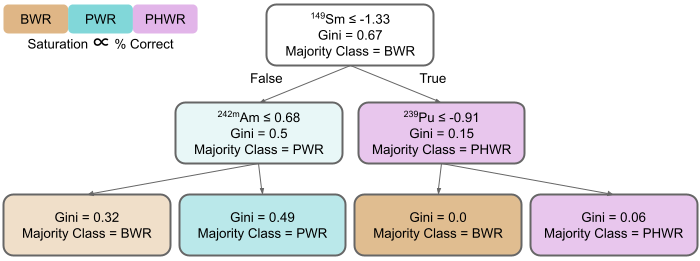
\includegraphics[width=\linewidth]{./chapters/litrev/dtree.png}
  \caption{Example of a decision tree process, where maximum tree depth was 
           limited to 2 for vizualization purposes.}
  \label{fig:dtr}
\end{figure}

In Figure \ref{fig:dtr}, the first split is determined to occur at the feature
Sm149 on whether the nuclide measurement is above a value of $-1.33$. Note that
this value is negative because of the scaling process the training set is put
through, described in Section \ref{sec:statmodel1}. The majority class at this
node is \gls{BWR} which is expected since the training set is 72\% \gls{BWR}.
The values list indicates the fraction of each class in the node, which is
alphabetically ordered \texttt{[bwr, phwr, pwr]}. It is even among the three
because the class weights were told to be balanced.  This splitting criterion
provides a Gini impurity score of 0.67, which represents the minimum Gini
impurity of all the candidate splits, but also indicates there are multiple
classes represented in this node (again, expected).  It would be 0 if there
were only one class in the node.  In the visualization, the shading of the
colors in the tree are bolder for there being a higher fraction of a single
class.

\subsubsection{Maximum Log-Likelihood Calculations}

The \gls{MLL} calulations approach applied here is based on a method developed
to do similar work \cite{mll_method, mll_validate, mll_sensitivity}.  That work
involved matching nuclear material samples based on some select measurements to
entries in a database of containing those measurements (see Section
\ref{sec:stats4nf}).  Each database entry also has a similar list of labels to
the labels being predicted in this work: reactor type, burnup, and time since
irradiation.

Interestingly, the \gls{MLL} calculations method works like \textit{k}-nearest
neighbors, where there is no model but a prediction according to the closest
match database entry.  There is one detail that differs, however. Whereas
\textit{k}-nearest neighbors minimizes distance/dissimilarity, this approach
instead maximizes similarity via a likelihood function. An "unknown" test
sample is compared against the training set using the likelihood calculation
between that sample and the training set entries.  The higher the likelihood,
the higher the probability that the database entry represents the sample. The
likelihood is in Equation \ref{eq:like}, whereas the log-likelihood is used
more often in practice, shown in Equation \ref{eq:loglike}.
\begin{equation}
  L(M|x_{test}) = \prod_i \frac{1}{\sigma_{i,train} \sqrt{2\pi}} \exp{\frac{-(x_{i,test} - x_{i,train})^2}{2 \sigma_{i,train}^2}}
  \label{eq:like}
\end{equation}
\begin{equation}
  ln(L(M|x_{test})) = \sum_i ln(\frac{1}{\sigma_{i,train} \sqrt{2\pi}}) - \frac{(x_{i,test} - x_{i,train})^2}{2 \sigma_{i,train}^2}
  \label{eq:loglike}
\end{equation}
The likelihood is a measure of the probability that a model $M$ produced the
measurements seen in the test sample, given by $L(M|x_{test})$.  In both
Equations \ref{eq:like} and \ref{eq:loglike}, $x$ refers to the set of
features, and $x_{i, test}$ and $x_{i,train}$ are the individual features for the
test sample and the training set entries, respectively. The uncertainty of the
measurement associated with each feature is represented by $\sigma_{i,train}$.


\subsection{Performance Evaluation \& Metrics}

\begin{frame}
  \frametitle{Testing Protocol}
  \begin{adjustwidth}{-15pt}{0pt}
  \vspace{-5pt}
  \begin{block}{Scikit-Learn Algorithms:}
    \begin{enumerate}
      \itemsep 0.2em 
      \footnotesize
      \item Scale training data ($0$ mean and unit variance)
      \item 5-fold cross val is used to iteratively remove 20\% of the train-set as a test-set
      \item \texttt{fit} and \texttt{predict} takes place, ground truth and predictions are tracked
      \item Each label is predicted separately
    \end{enumerate}
  \end{block}
  \pause
  \vspace{-5pt}
  \begin{block}{Maximum Log Likelihood:}
    \begin{enumerate}
      \itemsep 0.2em 
      \footnotesize
      \item Training database broken up into 10k segments (CHTC)
      \item Every training database entry is tested
      \item Testing sample removed from DB during each calculation
      \item Entire set of labels (reactor type, burnup, etc) predicted at once
    \end{enumerate}
  \end{block}
  \pause
  \vspace{-5pt}
  \begin{block}{SFCOMPO Testing with Nuclide Mass Training Set:}
    \begin{enumerate}
      \itemsep 0.2em 
      \footnotesize
      \item After filtering out for irrelevant cases, 505 test entries remain
      \item Training set units are converted to $mg/gU_i$
      \item In scikit, scaling is applied to the training set and testing set features
      \item MLL converts the units but doesn't require scaling
      \item Time since irradiation not included in SFCOMPO
    \end{enumerate}
  \end{block}
  \end{adjustwidth}
\end{frame}

\begin{frame}
  \frametitle{Reactor Type Classification Performance}
  \textbf{Accuracy Metrics:} \cite{scikit}
  \vspace{2mm}
  \begin{itemize}\addtolength{\itemsep}{0.4\baselineskip}
    \item $\uncover<1->{\textit{accuracy} = }
           \uncover<4->{\frac{1}{N_\text{samples}}}
           \uncover<3->{\sum_{i=1}^{N_\text{samples}}}
           \uncover<2->{\mathbb{I}(y_{pred,i} = y_{true,i})}$
    \item $\uncover<1->{\textit{balanced-accuracy} = }
           \uncover<5->{\frac{1}{\sum_{i}{w_i}}}
           \uncover<3->{\sum_{i=1}^{N_\text{samples}}}
           \uncover<5->{w_i \cdot}
           \uncover<2->{\mathbb{I}(y_{pred, i} = y_{true, i})}$ \\
          \hspace{1.1cm} \uncover<6->{where: $w_i = \frac{1}{\sum_j{\mathbb{I}(y_j = y_i)w_j}}}$
    \uncover<7->{\item Confusion matrices:}
  \end{itemize}
  \invisible<-6>{\begin{figure}
    \centering
    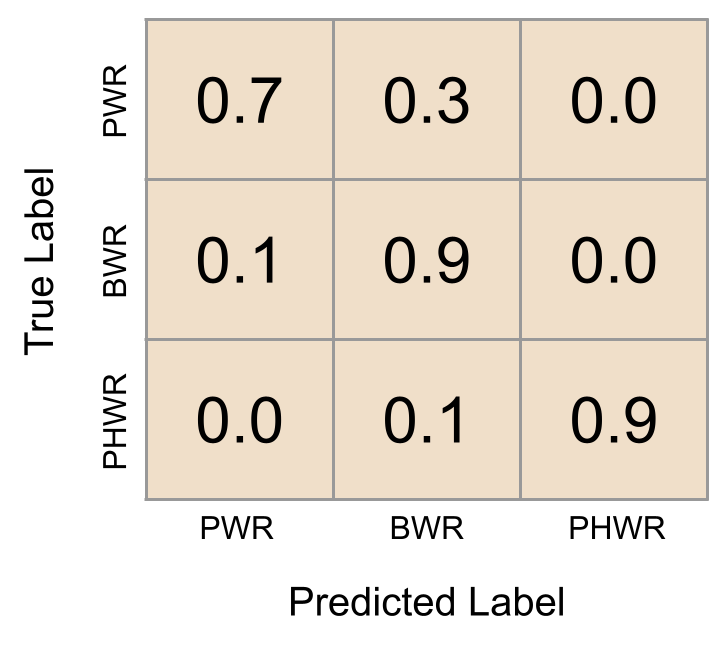
\includegraphics[width=0.35\linewidth]{./figures/cm_example.png}
  \end{figure}}
\end{frame}

\begin{frame}
  \frametitle{Performance Measures for Regression}
  \textbf{Regression Metrics:} \cite{scikit}
  \vspace{2mm}
  \begin{itemize}\addtolength{\itemsep}{0.4\baselineskip}
    \item \uncover<1->{Mean Absolute Error:\\ \vspace{2mm}
          $\textit{MAE} = \frac{1}{N_{\text{samples}}} \sum_{i=1}^{N_{\text{samples}}} \left| y_{true, i} - y_{pred, i} \right|$}
    \item \uncover<2->{Median Absolute Error:\\ \vspace{2mm}
          $\textit{MedAE} = \text{median}(\mid y_{true, 1} - y_{pred, 1} \mid, \ldots, 
                                          \mid y_{true, n} - y_{pred, n} \mid)$}
    \item \uncover<3->{Mean Absolute Percentage Error:\\ \vspace{2mm}
          $\textit{MAPE} =  \frac{100}{N_{\text{samples}}} \cdot 
                            \sum_{i=1}^{N_{\text{samples}}}
                            \frac{\left| y_{true, i} - y_{pred, i} \right|}{y_{true, i}}$}
  \end{itemize}
\end{frame}



\section{Reactor Operation Parameter Prediction Results}
\subsection{Prediction Performance using Nuclide Masses}
\begin{frame}
  \frametitle{Reactor Type Classification}
    \begin{figure}
      \centering
      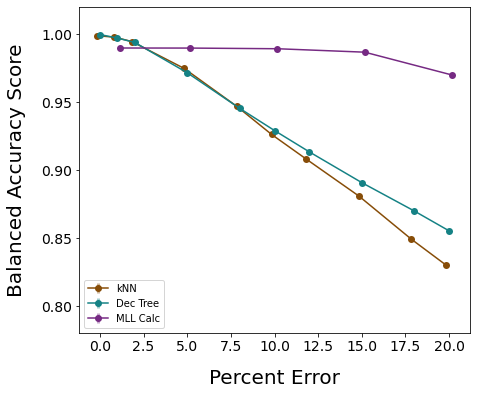
\includegraphics[width=0.6\textwidth]{./figures/randerr_compare_nuc29_BalAcc_rxtr.png}
      \caption{Reactor type prediction (balanced) accuracy using 29 nuclide masses for 3 algorithms}
    \end{figure}
\end{frame}

\begin{frame}
  \frametitle{Reactor Type Classification}
    \begin{figure}
      \centering
      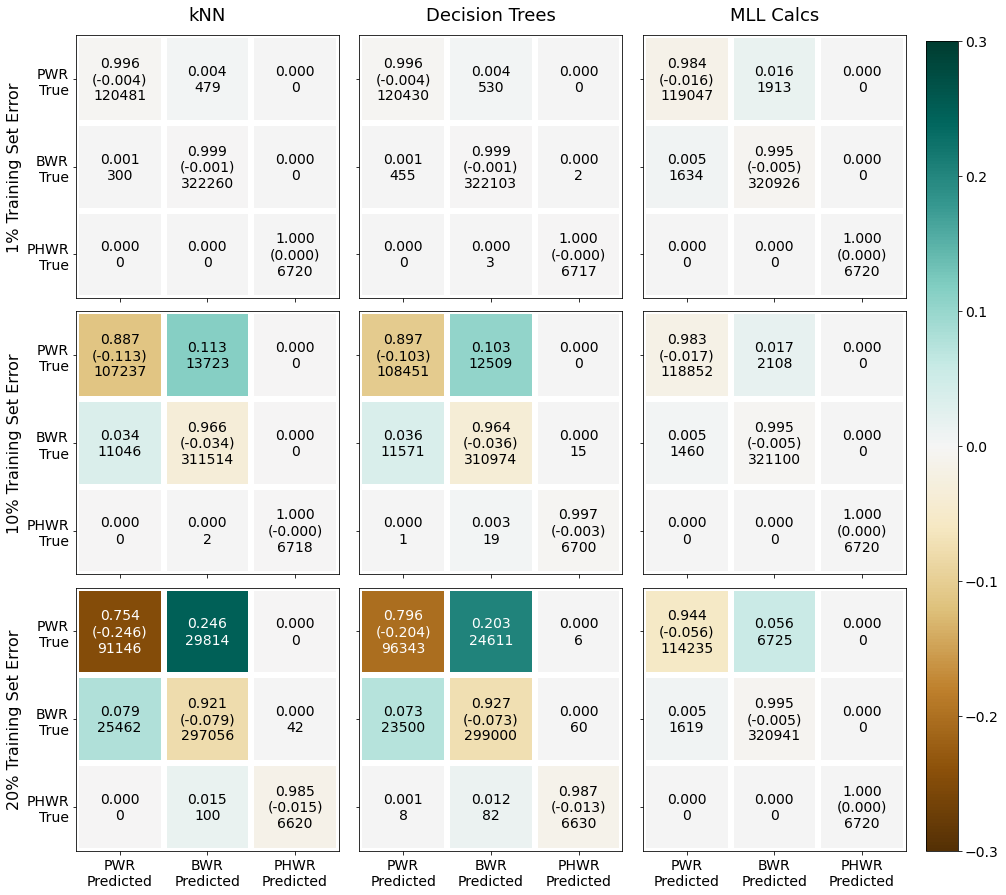
\includegraphics[height=0.75\textheight]{./figures/confusion_matrix_nuc29_3errs.png}
      \caption{Confusion matrices for three algorithms at three error levels}
    \end{figure}
\end{frame}

  %\begin{adjustwidth}{-15pt}{0pt}
  %\begin{minipage}{0.5\textwidth}
  %\end{minipage}%
  %\hfill
  %\begin{minipage}{0.5\textwidth}
  %  \begin{figure}
  %    \centering
  %    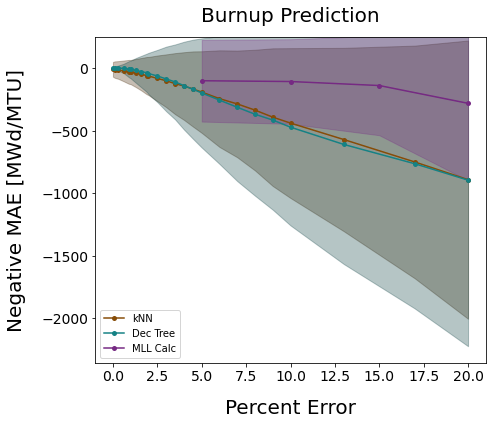
\includegraphics[width=1.08\linewidth]{./figures/randerr_compare_nuc29_burn.png}
  %    \caption{Burnup mean absolute prediction error using 29 nuclide masses for 3 algorithms}
  %  \end{figure}
  %\end{minipage}
  %\end{adjustwidth}
%\begin{frame}
%  \frametitle{Predictions with Random Error}
%  \begin{adjustwidth}{-15pt}{0pt}
%  \begin{minipage}{0.5\textwidth}
%    \begin{figure}
%      \centering
%      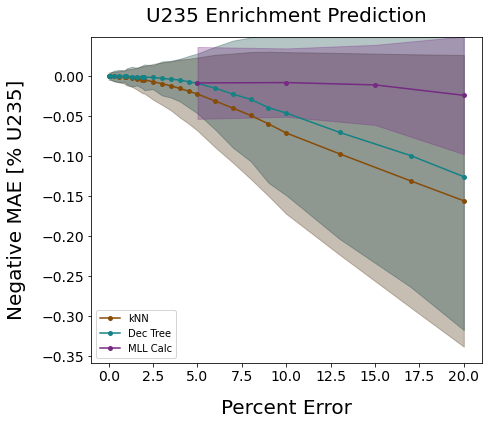
\includegraphics[width=1.08\linewidth]{./figures/randerr_compare_nuc29_enri.png}
%      \caption{U235 enrichment mean absolute prediction error using 29 nuclide masses for 3 algorithms}
%    \end{figure}
%  \end{minipage}%
%  \hfill
%  \begin{minipage}{0.5\textwidth}
%    \begin{figure}
%      \centering
%      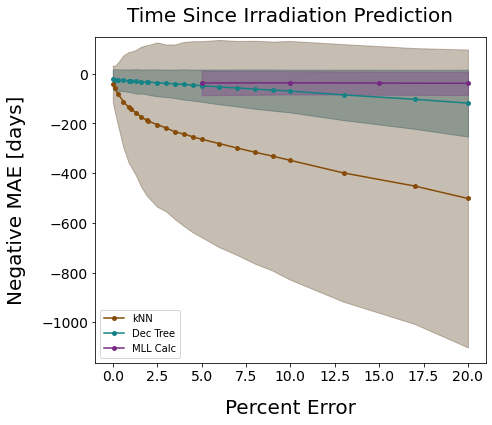
\includegraphics[width=1.08\linewidth]{./figures/randerr_compare_nuc29_cool.png}
%      \caption{Time since irradiation mean absolute prediction error using 29 nuclide masses for 3 algorithms}
%    \end{figure}
%  \end{minipage}
%  \end{adjustwidth}
%\end{frame}

\begin{frame}
  \frametitle{Predictions of SFCOMPO Test Cases}
  \begin{adjustwidth}{-15pt}{0pt}
  \begin{minipage}{0.85\textwidth}
    \begin{itemize}
      \item 505 test cases in total 
      \item Most test samples have many features missing (see table to left)
      \item Scikit algs don't handle null values, so the missing nuclide measurements are replaced with $0$
    \end{itemize}
    \bigskip
    \begin{table}
      %\centering
      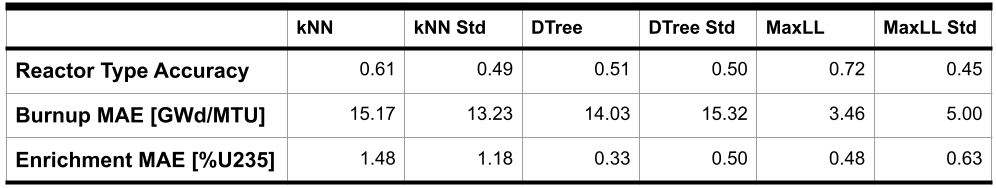
\includegraphics[width=\textwidth]{./figures/sfcompo_pred_results.png}
      \caption{Accuracy (not balanced) and mean absolute errors of the test cases in the SFCOMPO database}
    \end{table}
  \end{minipage}%
  \hfill
  \begin{minipage}{0.15\textwidth}
    \begin{table}
      %\centering
      
\includegraphics[height=0.89\textheight]{./figures/sfcompo_nuc_counts.png}
      %\caption{The number of entries that includes a measurement for each nuclide}
    \end{table}
  \end{minipage}
  \end{adjustwidth}
\end{frame}

\subsection{Prediction Performance using Processed Gamma Spectra}
\begin{frame}
  \frametitle{Predictions with Decreasing Detector Energy Resolution}
  \begin{adjustwidth}{-25pt}{0pt}
  \begin{figure}
    \centering
    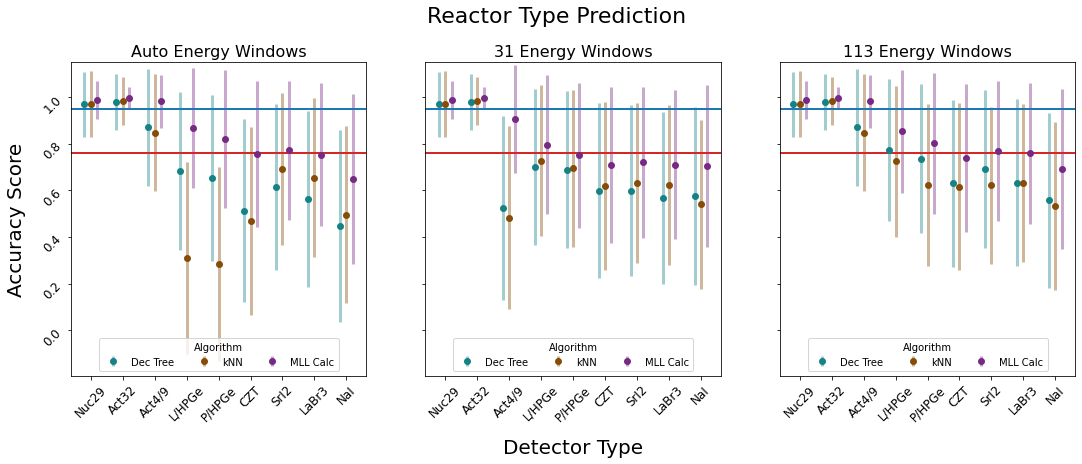
\includegraphics[width=1.15\textwidth]{./figures/detector_preds_wrt_enlist_reactor.png}
    \caption{caption}
  \end{figure}
  \end{adjustwidth}
\end{frame}

\begin{frame}
  \frametitle{Predictions with Decreasing Detector Energy Resolution}
  \begin{adjustwidth}{-25pt}{0pt}
  \begin{figure}
    \centering
    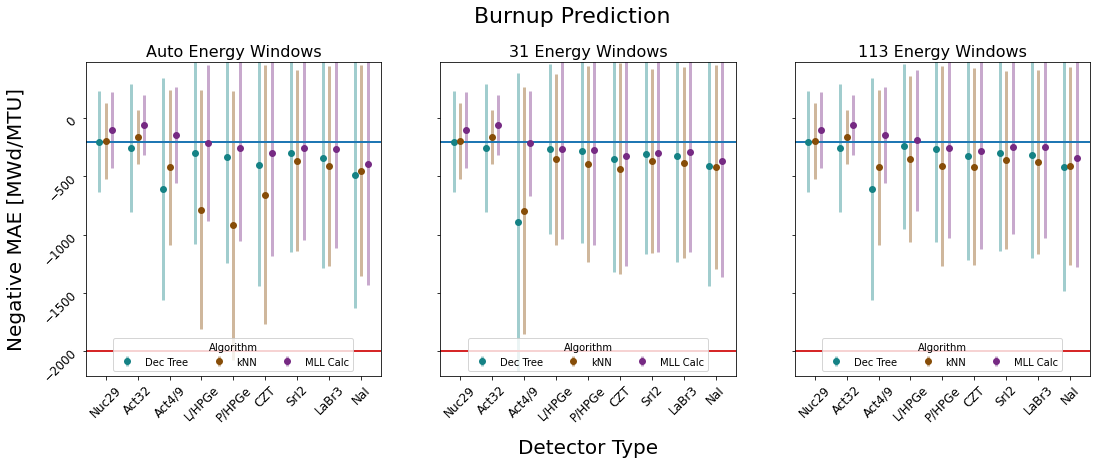
\includegraphics[width=1.15\textwidth]{./figures/detector_preds_wrt_enlist_burnup.png}
    \caption{caption}
  \end{figure}
  \end{adjustwidth}
\end{frame}

\begin{frame}
  \frametitle{Predictions with Decreasing Detector Energy Resolution}
  \begin{adjustwidth}{-25pt}{0pt}
  \begin{figure}
    \centering
    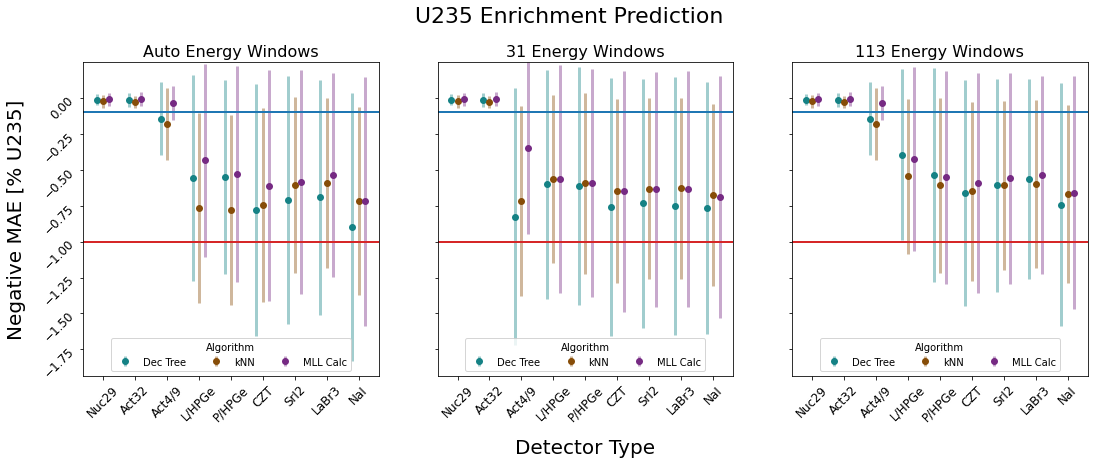
\includegraphics[width=1.15\textwidth]{./figures/detector_preds_wrt_enlist_enrichment.png}
    \caption{caption}
  \end{figure}
  \end{adjustwidth}
\end{frame}

\begin{frame}
  \frametitle{Predictions with Decreasing Detector Energy Resolution}
  \begin{adjustwidth}{-25pt}{0pt}
  \begin{figure}
    \centering
    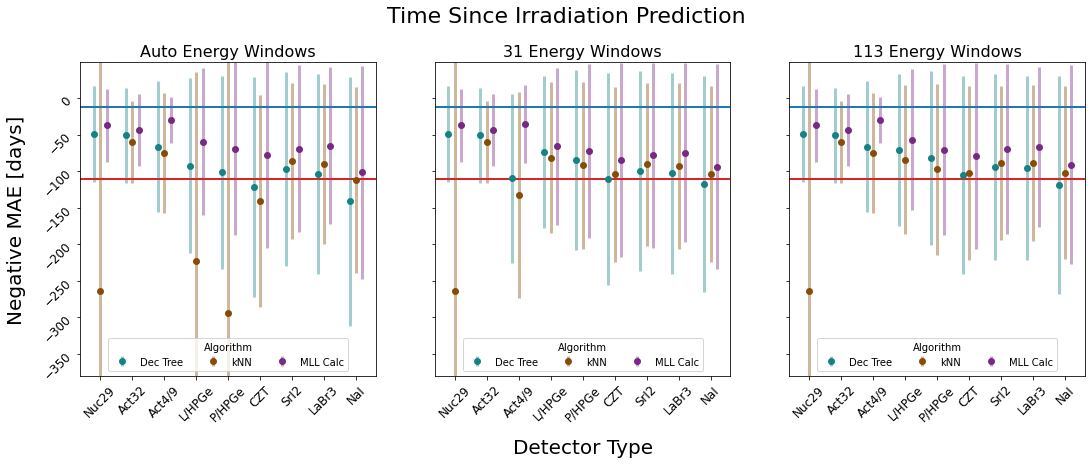
\includegraphics[width=1.15\textwidth]{./figures/detector_preds_wrt_enlist_cooling.png}
    \caption{caption}
  \end{figure}
  \end{adjustwidth}
\end{frame}



\section{Summary}
\subsection{Conclusions \& Future Work}

\begin{frame}
  \frametitle{Summary: Experimental Design Overview}
  \begin{adjustwidth}{-15pt}{-10pt}
  \textbf{Pre-detonation nuclear forensics analysis on SNF}\\
  \vspace{2pt}
  \begin{minipage}{0.38\textwidth}
    \begin{figure}
      \centering
      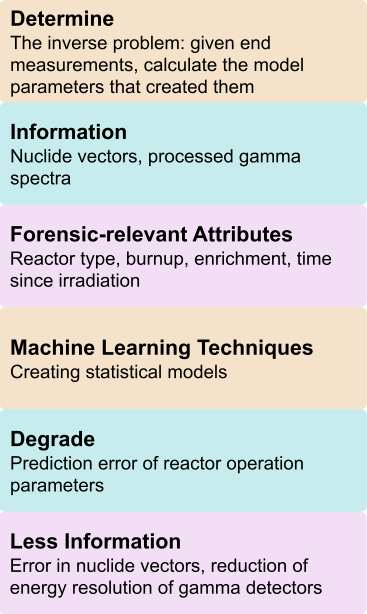
\includegraphics[height=0.78\textheight]{./figures/overview.png}
    \end{figure}
  \end{minipage}%
  \hfill
  \begin{minipage}{0.65\textwidth}
    \begin{block}{Main Goal:}
      \small
      Is it possible to speed up a nuclear forensics investigation of spent
      nuclear fuel with field-deployable detection?
    \end{block}
    \vspace{-8pt}
    \begin{block}{Demonstrated:}
      \small
      \begin{itemize}
        \itemsep 0.1em 
        \item Simulation of training data set
        \item Information reduction of training set
        \item Prediction of reactor type, burnup, enrichment, and time since irradiation via:
          \begin{itemize}
            \item \textit{k}-Nearest Neighbors
            \item Decision Trees
            \item Maximum Log-Likelihood Calculations
          \end{itemize}
        \item Evaluation of predictions with respect to information reduction
      \end{itemize}
    \end{block}
  \end{minipage}
  \end{adjustwidth}
\end{frame}

\begin{frame}
  \frametitle{Conclusions}
  \begin{itemize}
    \item Experiment 1: Nuclide Masses
      \begin{itemize}
        \item Difficult to judge performance baseline, chose generous "standard" from nuclide mass results
        \item SFCOMPO is challenging with this methodology but improvements can be made
      \end{itemize}
    \item Experiment 2: Processed Gamma Spectra
      \begin{itemize}
        \item Burnup is the only parameter to be well-predicted with gamma spectra
        \item ${}^{235}\text{U}$ enrichment is the only parameter to have very poor performance with gamma spectra
      \end{itemize}
    \end{itemize}
\end{frame}

\begin{frame}
  \frametitle{Future Work}
  \begin{itemize}
    \item Based on simplifications in this work
      \begin{itemize}
        \item Simulation fidelity (ORIGEN-ARP, homogenized core)
        \item Deeper study on gamma spectra processing
        \item Deeper inquiry into feature reduction
      \end{itemize}
    \item Based on questions this work raised
      \begin{itemize}
        \item Serial prediction, with detailed classification accuracy study 
        \item SFCOMPO improvements, novel imputation approach
        \item Could other statistical methods perform better? Would MLL with $k>1$ perform better?
      \end{itemize}
    \end{itemize}
\end{frame}


\subsection{Acknowledgements}
This proposal would not be possible with the wisdom and patience of my advisor,
Paul Wilson. I honestly don't have words for how grateful I am to you.  I'm
also appreciative of the CNERG community for technical and non-technical
assistance; may quiche recipes be forever shared during important phone calls.
Kelly Burton and Max Lagally have invested much effort into my success and
convinced me that graduate school was the right path for me---more than once.
My GERS friends have given me so much in and out of school, especially Jos\'e
Roberto, Richard, and Chandler.  I have also received generous funding from the
National Science Foundation and the Department of Homeland Security.

Mountains of personal support motivated me here and kept me here, which I do
not take for granted. Steven W. Harrell, my chosen family, inspired me to get
all my KSAs, no matter where I wanted to find them. The "If you're gonna be
dumb, you gotta be tough" mentality hilariously applies to a PhD program.
Robin, you have been such a light in my life for over a decade and always
remind me why I came back to grad school.  And to my friends for 15 years,
thanks for keeping in touch despite the gaps.  Denise and April, it's been
amazing to watch your wonderful transformations. Ruthie, you push me to be
fierce, spittin' truths and slaying your way through life.  Maurice, thanks for
the help when I was struggling. Lou, thanks for being one of my best friends
and sources of laugh lines. Liz, I love finding your inspirational notes around
my home and thanks for all the meals. For endlessly encouraging my academic
pursuits, I'm appreciative of my California family, Mel, Bonnie, Joelle, and
Jamie. Finally, my Madison family has blessed me in countless ways: Shan,
Ninja, Peter, Drax, Heather, Burnie, Marit, Sarah, James, BLou, Fetal, Matt, 



%%--------------------------------%%
%%--------------------------------%%

\begin{frame}[allowframebreaks]
  \frametitle{References}
  \bibliographystyle{plain}
  {\footnotesize \bibliography{pres} }
\end{frame}

%%--------------------------------%%

\end{document}


